\documentclass[12pt]{report}
\usepackage[pdftex]{graphicx}
\usepackage[margin=1.2in]{geometry}
\usepackage{listings}

% \usepackage{graphicx} %package to manage images
\graphicspath{{./images/}}

\begin{document}

\tableofcontents

\chapter{Week 1}

\section{Supervised and Unsupervised Learning}
The most basic thing to remember is that we already know what out correct output should look like in Supervised Learning.
But, we have little or no idea about what out results should look like.

\textbf{Supervised Learning:}
\begin{itemize}
	\item Classification: Spam/Not-spam. 
	\item Regression: Predicting age.
\end{itemize}

\textbf{Unsupervised Learning:}
\begin{itemize}
	\item Clustering: Grouping based on different variables.
	\item Non Clustering: Finding structue in chaotic environment.
\end{itemize}

\section{Linear Regression with one variable}
Regression being a part of Supervised Learning is used for estimatng data (Real-valued output).  

\subsection{Cost Function}
 This function measures the performance of a Machine Learning model for given data.

\textbf{Hypothesis}: $ h_ \theta(x) = \theta_0 + \theta_1x $

\textbf{Parameters:} $ \theta_0, \theta_1 $

\textbf{Cost Function:} 
\begin{equation} \label {eq:1}
	J( \theta_0, \theta_1 ) = 1/2m \sum_{i=1}^{m} (h_\theta(x^{(i)})-y^{(i)})^2 
\end{equation} 

\textbf{Goal:} Minimize cost function with $ \theta_0, \theta_1 $ as parameters.

\subsection{Gradient Descent}

\textbf{Basic idea:}
\begin{itemize}
\item Start with some $ \theta_0, \theta_1 $
\item Keep changing $ \theta_0, \theta_1 $ to reduce $ J(\theta_0, \theta_1) $ until we end up at minima.
\end{itemize} 

\textbf{Algorithm:}
 repeat until convergence:
\begin{equation} \label {eq:2}
	\theta_j := \theta_j - \alpha \frac{\partial {J(\theta_0, \theta_1)}}{\partial \theta_j}
\end{equation} 

(for  $j = 0, 1 $  ,here).	

\textbf{Intution:} 
If $\alpha$ is too small, descent can be slow and if too large, descent may fail to converge or even diverge.
Gradient descent can converge to a local minimum, even with fixed learning rate $\alpha$. As we approach local mimimum, gradient descent will automatically take smaller steps. So, no need to decrease $\alpha$ over time. 

\subsection{Gradient Descent for linear regression}
Combining gradient descent algorithm with linear regression model, we get:

\begin{equation} \label {eq:3}
	j = 0 : \frac{\partial {J(\theta_0, \theta_1)}}{\partial \theta_0} = 1/2 \sum_{i=1}^{m} (h_\theta(x^{(i)})-y^{(i)}) 
\end{equation}

\begin{equation} \label {eq:4}
	j = 1 : \frac{\partial {J(\theta_0, \theta_1)}}{\partial \theta_1} = 1/2 \sum_{i=1}^{m} (h_\theta(x^{(i)})-y^{(i)}).x^{(i)}
\end{equation}

Now, we can repeat \ref{eq:3} and \ref{eq:4} until convergence to obtain the minima.

"Batch" gradient descent: Each step of gradient descent uses all the training examples.
For eq. "m" batches in equation \ref{eq:1}.




\chapter{Week 2}

\section{Multivariate Linear Regression}
Linear regression involving more than one variable. For eq., Predicting price of a house based on parameters "Plot Area", "No. of Floors", "Connectivity with markets", etc.

\subsection{Multiple Features}
The multivariable form of the hypothesis is as follows:
\begin{equation} \label {eq:5}
	h_\theta(x) = \theta_0 + \theta_1x_1 + \theta_2x_2 + \theta_ 3x_3 + ... + \theta_{n}x_n.	
\end{equation}
This hypothesis funtion can be concisely represented as:
\begin{equation}
	h_\theta(x) = \theta^{T}x
\end{equation}
where, $ \theta^T $ is a 1xn matrix consisting of $ \theta_0, \theta_1, \theta_2 ... \theta_n $.


\subsection{Gradient Descent for Multiple Variables}
Gradient descent formula for Multiple variable will be similar to that of single variable.

\begin{equation} \label {eq: GD for multiple}
	\theta_j =  \theta_j - \alpha \frac{1}{m} \sum_{i=1}^{m} (h_\theta(x^{(i)})-y^{(i)}).x_j^{(i)}
\end{equation}

Repeating this equation until convergence will give the minima. \footnote[1]{$x_0 = 1$ in equation \ref{eq: GD for multiple}}

\subsubsection{Feature Scaling}
Feature Scaling is used to reduce the number of iterations in Gradient Descent. Basic idea of feature scaling is to bring all the features on the same scale. (in general we try to approximate every feature in the range $ -1 < x_i < 1 $)
\\ \\ Reducing the number of iteration doesn't mean making computation of each step easier. And also it does not effect comtational efficiency of Normal Equation.

\subsubsection{Mean Normalisation}
Mean Normalisation makes features to have approximately zero mean.

\subsubsection{Learning Rate}
If $\alpha$ is too small: slow convergence.

if $\alpha$ is too large: $J(\theta)$ may not decrease on every iteration, or may not converge.

\subsubsection{Polynomial Regression}
Selecting proper polynomial for fitting data is very important.

\begin{figure}[h]
	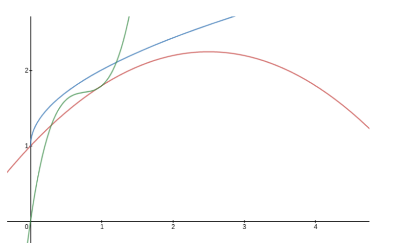
\includegraphics[width=8cm, height=5cm]{polyreg.png}
\end{figure}

\textbf{Red:} Quadratic

\textbf {Blue:} Square root funtion $ \theta_0+\theta_1x+\theta_2\sqrt{x} $

\textbf {Green:} Cubic function

\section{Normal equation}
Normal Equation is a method to solve for $\theta_T$ analytically, by creating a $m\times(n+1)$ matrix $X$ and another $m\times1$ matrix $Y$.\footnote[2]{Every element of first column of matrix $X$ is 1 and other are the feature's coefficient}

Mathematically $\theta$ is given as:
\begin{equation} \label {eq: theta}
	\theta = (X^TX)^{-1}X^ty
\end{equation}

\begin{tabular}{ |c|c|}
	\hline
	\textbf{Gradient Descent} & \textbf{Normal Equation} \\
	\hline
	Need to choose $\alpha$ & No need to choose $\alpha$ \\
	Needs many iteration & Don't need to iterate \\
	Works well with large n & Slow for large n \\
	\hline
\end{tabular}

\vspace{5mm}

\subsubsection{Reasons for non-invertiblity of $X^T X$}
\begin{itemize}
	\item Redundant features (linear dependence) \footnote[3]{Eg. Using both $m^2 \  \& \  (feet)^2$ features}
	\item Too many features (m $<=$ n) 
\end{itemize}

\section{Octave/MATLAB commands}

\subsubsection{Basic Operations}
\begin{lstlisting}[basicstyle=\small]
octave:1> a = pi
a =  3.1416
octave:2> disp(sprintf('6 decimals: %0.6f', a))
6 decimals: 3.141593
octave:3> a
a =  3.1416
octave:4> format long
octave:5> a
a =  3.141592653589793
octave:6> format short
octave:7> a
a =  3.1416
octave:8> v = 1:0.1:2
v =

    1.0000    1.1000    1.2000    1.3000    1.4000    1.5000    1.6000    1.7000    1.8000    1.9000    2.0000

octave:9> v = 1:0.1:2
v =

 Columns 1 through 8:

    1.0000    1.1000    1.2000    1.3000    1.4000    1.5000    1.6000    1.7000

 Columns 9 through 11:

    1.8000    1.9000    2.0000

octave:10> v = 1:6
v =

   1   2   3   4   5   6

octave:11> zeros(1,3)
ans =

   0   0   0

octave:12> rand(1,3)
ans =

   0.43623   0.76554   0.23635

octave:13> randn(1,3)
ans =

   0.5602642  -0.0043628   0.1344922

octave:14> w = -6 + sqrt(10)*(randn(1,10000))

octave:15> hist(w)
\end{lstlisting}

\begin{figure}[h]
	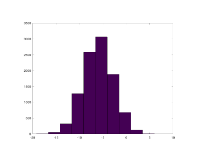
\includegraphics[width=4cm, height=3cm]{hist.png}
\end{figure}

\begin{lstlisting}[basicstyle=\small]
octave:1> w = -6 + sqrt(10)*(rand(1,10000));

octave:2> hist(w,50)
\end{lstlisting}

\begin{figure}[h]
	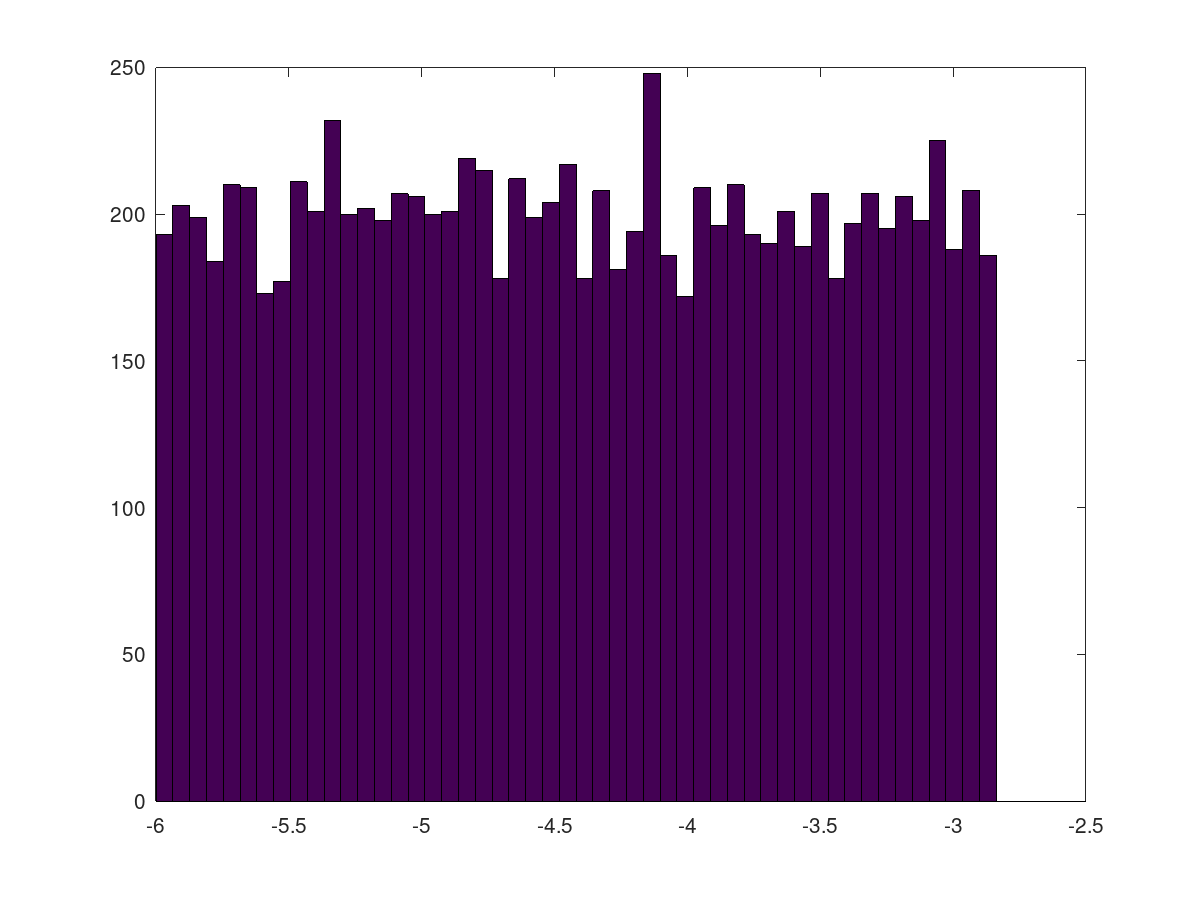
\includegraphics[width=4cm, height=3cm]{hist2.png}
\end{figure}

\subsubsection{Moving Data around}
\begin{lstlisting}[basicstyle=\small]
octave:1> A = [1,2;3,4;4,5]
A =

   1   2
   3   4
   4   5

octave:2> size(A)
ans =

   3   2

octave:3> sz = size(A)
sz =

   3   2

octave:4> size(sz)
ans =

   1   2

octave:5> size(A,1)
ans =  3
octave:6> size(A,2)
ans =  2
octave:7> length(A)
ans =  3
octave:8> length([1,2,3,4,5])
ans =  5
octave:9> 
octave:9> 
octave:9> pwd
ans = /home/sahasra
octave:10> cd /home/sahasra/
octave:11> pwd
ans = /home/sahasra
octave:12> ls
Android		       Documents	 Music	   Public     Videos
AndroidStudioProjects  Downloads	 MyPaint   snap
Desktop		       examples.desktop  Pictures  Templates
octave:13> who
Variables in the current scope:

A    ans  sz

octave:14> whos
Variables in the current scope:

   Attr Name        Size                     Bytes  Class
   ==== ====        ====                     =====  ===== 
        A           3x2                         48  double
        ans         1x13                        13  char
        sz          1x2                         16  double

Total is 21 elements using 77 bytes

octave:15> clear
octave:16> whos
octave:17> A = [1,2;3,4;5,6]
A =

   1   2
   3   4
   5   6

octave:18> A(3,2)
ans =  6
octave:19> A(2,:)
ans =

   3   4

octave:20> A(:,2)
ans =

   2
   4
   6

octave:21> A([1,3], :)
ans =

   1   2
   5   6

octave:22> A([2,3], :)
ans =

   3   4
   5   6

octave:23> A(:,2) = [10;11;12]
A =

    1   10
    3   11
    5   12

octave:24> A = [A, [5;6;7]]
A =

    1   10    5
    3   11    6
    5   12    7

octave:25> A(:)
ans =

    1
    3
    5
   10
   11
   12
    5
    6
    7

octave:26> A
A =

    1   10    5
    3   11    6
    5   12    7

octave:27> B = [45;46;47]
B =

   45
   46
   47

octave:28> C = [A,B]
C =

    1   10    5   45
    3   11    6   46
    5   12    7   47


\end{lstlisting}


\subsubsection{Computing on Data}
\begin{lstlisting}[basicstyle=\small]
octave:1> A = [1 2;3 4;5 6]
A =

   1   2
   3   4
   5   6

octave:2> B = [11 12; 13 14; 15 16]
B =

   11   12
   13   14
   15   16

octave:3> C = [1  1; 2 2]
C =

   1   1
   2   2

octave:4> A*C
ans =

    5    5
   11   11
   17   17

octave:5> A .* B % A .* B gives element wise operation
ans =

   11   24
   39   56
   75   96

octave:6> 1 ./ A
ans =

   1.00000   0.50000
   0.33333   0.25000
   0.20000   0.16667

octave:7> v = [1;2;3]
v =

   1
   2
   3

octave:8> log(v)
ans =

   0.00000
   0.69315
   1.09861

octave:9> exp(v)
ans =

    2.7183
    7.3891
   20.0855

octave:10> abs([-1; 2; -3])
ans =

   1
   2
   3

octave:11> A
A =

   1   2
   3   4
   5   6

octave:12> A' % A' = A transpose
ans =

   1   3   5
   2   4   6

octave:13> val = max([1;2;3;6;7])
val =  7
octave:14> max(A)
ans =

   5   6

octave:15> A
A =

   1   2
   3   4
   5   6

octave:16> a = [1;4;6;7;9]
a =

   1
   4
   6
   7
   9

octave:17> a < 3
ans =

  1
  0
  0
  0
  0

octave:18> find(a<3)
ans =  1
octave:19> A = magic(3) % Magic Square
A =

   8   1   6
   3   5   7
   4   9   2

octave:20> [r,c] = find(a >= 7)
r =

   4
   5

c =

   1
   1

octave:21> a
a =

   1
   4
   6
   7
   9

octave:22> a = a'
a =

   1   4   6   7   9

octave:23> sum(a)
ans =  27
octave:24> rand(3)
ans =

   0.272471   0.059338   0.757392
   0.414497   0.174242   0.354694
   0.811891   0.935437   0.956667

octave:25> A
A =

   8   1   6
   3   5   7
   4   9   2

octave:26> max(A,[],1)
ans =

   8   9   7

octave:27> max(A,[],2)
ans =

   8
   7
   9

octave:28> max(max(A))
ans =  9
octave:29> A
A =

   8   1   6
   3   5   7
   4   9   2

octave:30> pinv(A)
ans =

   0.147222  -0.144444   0.063889
  -0.061111   0.022222   0.105556
  -0.019444   0.188889  -0.102778

octave:31> temp = pinv(A)
temp =

   0.147222  -0.144444   0.063889
  -0.061111   0.022222   0.105556
  -0.019444   0.188889  -0.102778


octave:32> temp * A
ans =

   1.0000e+00   2.0817e-16  -3.1641e-15
  -6.1062e-15   1.0000e+00   6.2450e-15
   3.0531e-15   4.1633e-17   1.0000e+00

octave:33> % this is the 3x3 Identity matrix, 
           % not having exact values beacuse of variable overflow
\end{lstlisting}

\begin{lstlisting}[basicstyle=\small]
octave:1> t = [0:0.01:0.98];
octave:2> y1 = sin(2*pi*4*t);
octave:3> plot(t,y1)
\end{lstlisting}

\begin{figure}[h]
	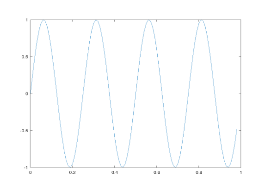
\includegraphics[width=6cm, height=4cm]{sineplot.png}
\end{figure}

\begin{lstlisting}[basicstyle=\small]

octave:4> y2 = cos(2*pi*4*t);
octave:5> plot(t,y1);
octave:6> hold on;
octave:7> plot(t, y2, 'r');
octave:8> xlabel('time')
octave:9> ylabel('value')
octave:10> legend('sin', 'cos')
octave:11> title('sine-cosine plot')
octave:12> print -dpng 'myPlot.png'
\end{lstlisting}

\begin{figure}[h]
	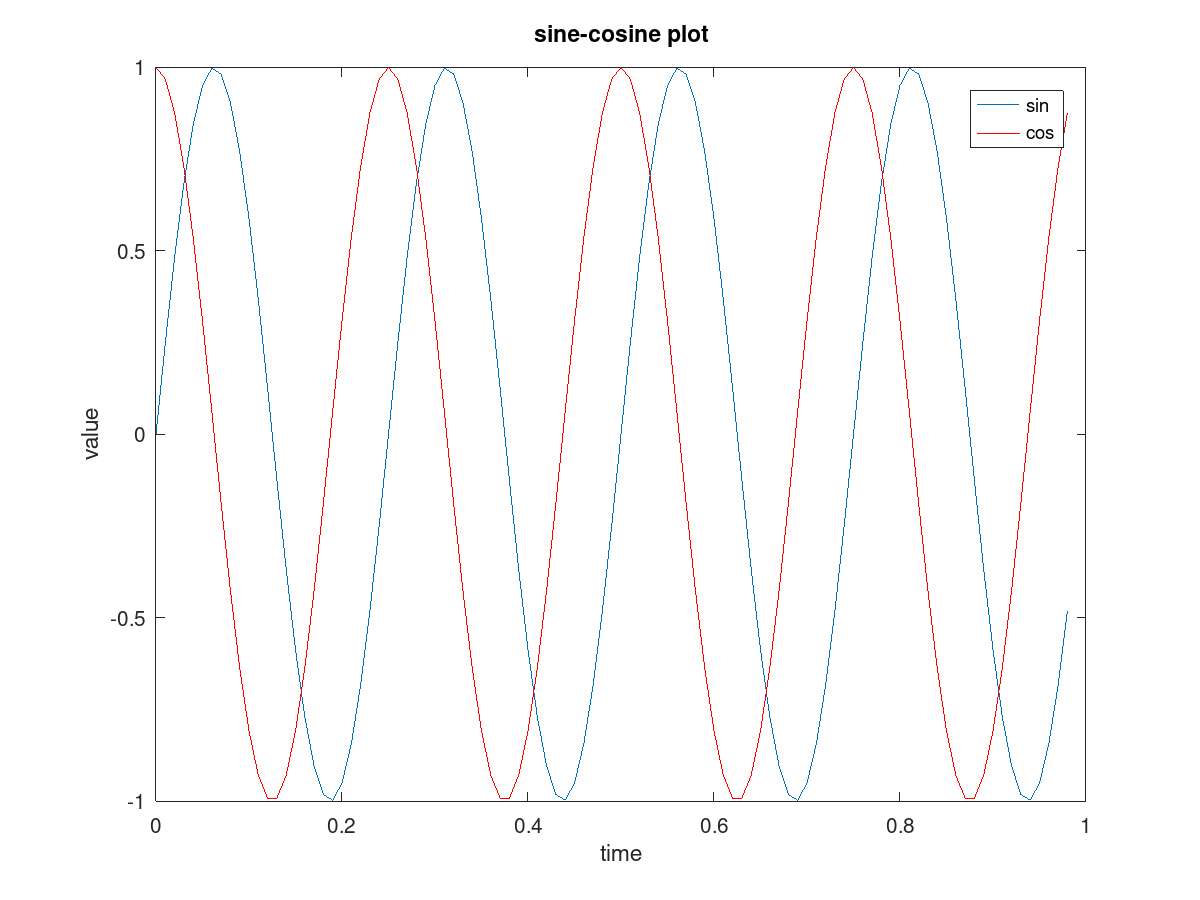
\includegraphics[width=6cm, height=4cm]{myPlot.png}
\end{figure}

\begin{lstlisting}[basicstyle=\small]

octave:13> close
octave:14> figure(1); plot(t, y1);
octave:15> figure(2); plot(t, y2);
octave:16> subplot(1,2,1);   % Divides plot a 1x2 grid
octave:17> plot(t,y1);
octave:18> subplot(1,2,2)
octave:19> plot(t,y2);
octave:20> axis([0.5 1 -1 1])
\end{lstlisting}

\begin{figure}[h]
	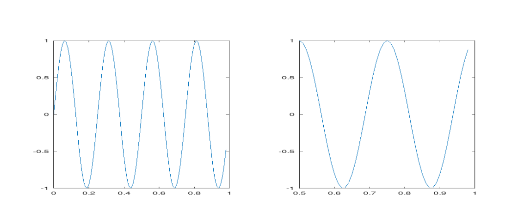
\includegraphics[width=12cm, height=4cm]{plot2.png}
\end{figure}

\vspace{5mm}
\subsubsection{Control Statements: for, while, if, else-if ...}

\begin{lstlisting}[basicstyle=\small]
octave:1> v = zeros(10,1)
v =

   0
   0
   0
   0
   0
   0
   0
   0
   0
   0

octave:2> for i=1:10,
> v(i) = 2^i;
> end;

octave:3> v
v =

      2
      4
      8
     16
     32
     64
    128
    256
    512
   1024

octave:4> i=1;
octave:5> while i <= 5,
> v(i) = 100;
> i = i+1;
> end;
octave:6> v
v =

    100
    100
    100
    100
    100
     64
    128
    256
    512
   1024

octave:7> i = 1;
octave:8> while true,
> v(i) = 999;
> i = i+1;
> if i == 6,
> 	break;
> end;
> end;

octave:9> v
v =

    999
    999
    999
    999
    999
     64
    128
    256
    512
   1024

\end{lstlisting}



\end{document}

